\documentclass[a4paper]{article}
\usepackage[utf8]{inputenc}

\usepackage{url}

\usepackage{titling}

\usepackage{titlesec}
\newcommand{\sectionbreak}{\clearpage}

\usepackage{amsmath,amssymb}
\DeclareMathOperator{\E}{\mathbb{E}}
\DeclareMathOperator{\argmax}{argmax}

\usepackage{textcomp}

\usepackage{enumitem}
\setlist{nosep}

\usepackage[]{algorithm}
\usepackage[]{algpseudocode}

\usepackage{graphicx}
\graphicspath{ {images/} }

\makeatletter
\newcommand{\StatexIndent}[1][3]{%
  \setlength\@tempdima{\algorithmicindent}%
  \Statex\hskip\dimexpr#1\@tempdima\relax}
\algdef{S}[WHILE]{WhileNoDo}[1]{\algorithmicwhile\ #1}%
\makeatother

% \makeatletter
% \def\BState{\State\hskip-\ALG@thistlm}
% \makeatother



\title{Training Computers to Build LEGO Models using Reinforcement Learning with Deep Q-Network}
\author{Jiaxing Tong }
\date{May 2017}

\begin{document}
    \pagenumbering{gobble}
    \maketitle
    
    \begin{abstract}
        This project shows a way to train a computer (agent) to
        build a LEGO model in a simulated LEGO environment 
        according to a given LEGO model or a picture. Deep Q-learning \cite{human-level,DQN}
        is an algorithm which combines deep learning and reinforcement
        learning and uses artificial neural networks to train the
        agent in a specific simulated environment. This project shows
        a way to build up a LEGO environment along with a suitable
        neural network. Then, by expanding the environment and
        upgrading the algorithm, the agent can finally build a 3D
        LEGO model according to a real-world picture. 	
    \end{abstract}
    
    \newpage
    \tableofcontents
    \newpage

    \pagenumbering{arabic}
    
    \section{Introduction}
        \subsection{Overview}
            As computer hardware has become much more powerful than that
            in the last decade, the high performance of computers gave
            rise to the popularity of machine learning, especially its
            uses in artificial intelligence. A group of scientists from
            DeepMind suggested a new way, which combined deep learning
            and reinforcement learning, to train an agent to learn to
            play Atari games \cite{intro-rl} in 2015. After \cite{intro-rl} had been published,
            many people tried to train computers to play different video
            games, such as games on Atari, Flappy Bird \cite{flappy-bird1,flappy-bird2}, etc., using
            this algorithm. However I believed that this algorithm had
            some other application, so I tried to create an agent to learn
            to build LEGO models. 
            
            This project shows a way to train an agent to learn to rig up a LEGO model in a simulated environment using as input only the rendered image of the model which the agent has currently built and a value given by a pre-defined reward function which evaluates the gap between current model and the target model. Initially, the agent is offered the exact bricks required to build the target model. This is in a similar way where people purchase a box of a LEGO model from a store, where the bricks in the box are exactly the bricks of which the model consists, and pour the bricks onto a table and then assemble them piece by piece. The agent may choose a brick to move one step at each time. 
            
            In the later stage, the agent was upgraded and was able to pick
            a best brick from a large pool of bricks with different colours
            and put it to the best place at each step. Compared to the previous
            procedure, this is more similar to the process where a LEGO expert
            who has enough LEGO bricks and uses them to build a model from
            scratch. 
            
            I also added some simple physics into the LEGO environment, and observed if the agent can also learn to rig up models in an environment which is closer to the real world. 
            
            Here follows a rough outline of how the agent works: 
            
            \begin{enumerate}[leftmargin=1.5cm]
                \item Initially, we have an untrained Q-network, a target
                model, a current model and a rendered image for each model.
                \item The agent chooses the best action according to the Q
                values given by the Q-network.
                \item The agent inputs the chosen action to the LEGO
                environment, and get a model after that action along with
                the rendered image of this model.
                \item The agent compares the model we get and the target
                model and gets a reward value from the reward function.
                \item Put the reward value and other useful information
                into the replay pool.
                \item If there are enough replays in the replay pool, update
                the Q-network using some randomly picked replays from the
                replay pool.
                \item Repeat step 2 to 6 until the agent is able to build the
                target model or a pre-set maximum number of steps has been reached.
            \end{enumerate}
            
        \subsection{Purpose}
            The purpose of this project is to design an artificial intelligence
            and a simulated LEGO environment, improve the reward function and upgrade
            the LEGO environment so that it is more similar to the way where humans
            play with LEGO. 
            
            Everyone may easily get a real-world picture of an object, but it’s hard
            for a person who is lacking designing skills to design a LEGO model using
            some software such as LEGO DIGITAL DESIGNER. The project also aims to find
            such a way that the agent would be able to build the LEGO model according
            to a real world picture of an object. In order to build a 3D model, the
            picture might be captured by a 3D camera (which gives the picture a depth
            channel), or the system might require a set of multi-view pictures as its
            input. There are still some imperfections in the system, which can be
            improved in the future.
            
        \subsection{Project Road Map}
            This project aims to build up a complete system consisting of main codes,
            a neural network, a simulated LEGO environment and a rendering program.
            As the goal of this project is very ambitious and the whole system is
            complicated, I built the system part by part and upgraded some modules
            to improve the performance. 
            
            I will now explain the whole system in the following order. 
            
            Firstly, in the `Background' section, I will define some symbols which
            will be used in the rest part of the report I will also introduce some
            essential background knowledge of reinforcement learning as it is not
            fully covered in the machine learning course. Then, I will explain deep
            reinforcement learning, the most important algorithm in the whole system. 
            
            In the `Design' section, I will give a graphical overview of the entire
            system which reflects the inter-communication between each module and
            the outline of the algorithm. Then I will explain how the whole system
            works, how the neural network has been constructed, and how the individual
            modules work, the roles they play and how do they interact with each other.
            Moreover, if some modules have been upgraded, I will explain the reason why
            I upgraded them and the improvement after the upgrade. 
            
            Having explained the whole system, I will show some testing results and
            analyse the results to show the actual improvement of the system. Finally,
            I will draw conclusions from the results and the analysis that I have done,
            and then reveal some imperfections which can be further improved.





    \section{Background}
    
        \subsection{Definition}
        
        (Here I will include some symbols which I use in the report. Not finished.)
        action space
        
        action
        
        state space
        
        state
        
        value in rl
        
        optimal value in rl
        
        policy
        
        reward
        
        reward for an action
        
        overall reward
        
        Q values
        
        
        
        
        
        
        
        \subsection{Reinforcement Learning}
            In machine learning, reinforcement learning is an area
            inspired by behaviourist psychology \cite{thorndike1898animal}
            and neuroscience \cite{Schultz_1997}. It concerns how agents may take
            actions in an environment corresponding to the responses of
            the environment so as to maximise the total reward \cite{intro-rl}.
            The whole process mimics how animals learn to react to
            an environment.
            
            A reinforcement learning model consists of: \cite{intro-rl}
            \begin{enumerate}[leftmargin=1.5cm]
                \item a set of environment states $S$;
                \item a set of actions $A$;
                \item rules of transitioning between states;
                \item rules that determine the scalar immediate reward
                of a transition; and
                \item rules that describe what the agent observes.
            \end{enumerate}
            
            
            Assume the problem is episodic. An episode starts when the
            problem starts in an initial state and ends when some terminal
            states is reached. We also assume each episode is finite. In
            other words, whichever the actions are taken by the agent, 
            the problem always terminates at some point. We define a policy
            as a mapping to some probability distribution over all possible
            actions. Hence, the expectation of the total reward for any
            policy is well-defined.
            
            The expected return $\rho^\pi$ to policy $\pi$ is:
            \begin{equation*}
                \rho^\pi = \E [R|\pi]
            \end{equation*}
            where the return value R is defined by:
            \begin{equation*}
                R=\sum_{t=0}^{N-1} r_{t+1}
            \end{equation*}
            where $r_{t+1}$ is the immediate reward after the $t$-th transition. Here, $N$ denotes the time step when a terminal state is reached. \cite{intro-rl} Sometimes, in order to control the number of steps, the reward at each step can be multiplied by a discount factor $\gamma$, so R can also be defined by:
            \begin{equation*}
                R=\sum_{t=0}^{N-1} \gamma r_{t+1}
            \end{equation*}
            
            There are many algorithms for reinforcement learning \cite{intro-rl}. In this project, \textbf{Value Function approaches} is related to Deep Q-Learning algorithm.
            
            Value function approaches aim to find a policy which maximises the overall reward value. 
            
            Let $V^*$ be the optimality and it is defined as:
            
            \begin{equation*}
                V^*(s) = \max_\pi V^\pi (s)
            \end{equation*}
            where $V^\pi$ denotes the value of a policy $\pi$:
            
            \begin{equation*}
                V^\pi(s) = \E[R|s,\pi]
            \end{equation*}
            where $R$ is the random return with respect to the policy $\pi$ from the initial state $s$.
            
            Moreover, the state-values can be updated to action-values, and the algorithm becomes Q-Learning.\cite{Watkins:1989} And the Q-values are defined as:\cite{Q-l}
            
            \begin{equation*}
                Q^\pi(s,a) = r_s(a) + \gamma \sum_{a'}\E[s,a'|\pi]V^\pi(a').
            \end{equation*}
        
        
        
        \subsection{Deep Learning}
        
            Deep Learning is a class of machine learning in which artificial neural networks (also known as neural networks) are used to extract and transform features from raw data. A neural networks is a flow of many layers, and each layer consists a lot of non-linear processing units which are also called as nodes or neurons. Each neural network has an input layer, an output layer and one or more hidden layers. \cite{deep-learning-methods-and-applications,Deep-Learning, Schm14}
            
            In a neural network, neurons in the input layer receive the input data and output to next layer. Neurons in a hidden layer receive the output from the previous layer, and output values after some linear or non-linear transformations, according to parameters of neurons, to the next layer. And finally, the output layer receives values and output to the user. \cite{Deep-Learning,Schmidhuber_2015,Schm14,deep-learning-methods-and-applications,Bengio_2009}
            
            In this project, a deep neural network is used to simulate a function which returns Q values\cite{human-level}, so the network is also called Q-network.
            
            
            
            
            
            
            
            
            
        
        
        
        \subsection{Deep Reinforcement Learning, Deep Q-Learning and Deep Q-Networks}
        
            Deep Reinforcement Learning (also known as Deep Q-learning) is an 
            machine learning algorithm which was posted by DeepMind on their 
            website in 2013. \cite{Deep-RL} DeepMind then published an article about deep 
            reinforcement learning in Nature in 2015. \cite{human-level} In this article, they described
            an algorithm called Deep Q-network implemented deep reinforcement learning.
            
            Deep Reinforcement Learning is a combination of Deep Learning
            and Reinforcement Learning, which integrates both their features. 
            DeepMind wanted to use Deep Reinforcement Learning to create artificial
            agents which achieve a similar level of performance and generality.
            The Agents learn by themselves to achieve successful strategies leading
            to a greatest long-term rewards (feature of reinforcement learning) and
            learn their own knowledge directly from raw inputs, such as vision 
            (feature of deep learning). \cite{DQN}
            
            In Deep Q-learning, we are not concerning immediate reward values for each transition,
            but we are trying to maximise long-term reward values. There is also a set of Q-values for each state-action pair. Therefore a Deep Q-learning model
            consists of:
            \begin{enumerate}[leftmargin=1.5cm]
                \item a set of environment states $S$;
                \item a set of actions $A$;
                \item a set of Q-values $Q$;
                \item rules of transitioning between states;
                \item rules that determine the scalar immediate reward
                of a state from the nearest final state; and
                \item rules that describe what the agent observes.
            \end{enumerate}
            
            The agent is able to do some action in the environment; the agent can perceive any
            feedback from the environment; and most importantly, the agent has a Q-network,
            which takes the feedback as an input and outputs values for different actions.
            The agent can then take the best action accordingly. 
            
            The whole process simulates humans (or other animals). When humans are in an
            environment, humans are able to do some action in the environment; humans can perceive any feedback from the environment by means of senses of sight, hearing, touch (maybe taste and smell); and humans have brains which collect the information from sense organs and tell bodies to take some reactions.
            
            With this in mind, we may consider the problem in which the agent interacts with the environment. The agent receives an observation from the environment, selects an action, receives a reward from the environment, then receives the next observation and keeps doing these. The goal of the agent is to select actions at each state so that it can maximise cumulative future reward. \cite{human-level} We achieve this by using the Q-network. The Q-network is a deep convolutional neural network which approximates the optimal action-value function
            
            \begin{equation*}
                Q^*(s,a) = \max_\pi \E[r_t+\gamma r_{t+1}+ \gamma^2 r_{t+2}+...|s_t=s, a_t=a, \pi]
            \end{equation*}
            which maximises the overall rewards discounted by $\gamma$ at each time step $t$. This is achieved by a behaviour policy $\pi = P(a|s)$, after an observation $s$ and taking an action $a$.\cite{human-level}
            
            The agent has a limited memory to store replays (experiences). Each replay is a tuple $e_t = (s_{t}, a_t, r_t, s_{t+1})$ where $s_{t}$ is the state at time t, $a_t$ is the action taken after $s_t$, $r_t$ is the reward after $a_t$ had been taken, and $s_{t+1}$ is the state after $a_t$ had been taken from $s_t$. All the replays $e_1$ to $e_t$ are stored in a replay pool $D_t$.  When the number of replays in the pool reaches a threshold, the agent can uniformly pick one or more of these replays, wrap them as a mini-batch and train the Q-network with the mini-batch. 
            
            During learning, Q-learning updates are applied on the mini-batch. For each iteration $i$ the following loss function is used to update the Q-network:
            
            \begin{equation*}
                L_i(\theta_i) = \E_{(s,a,r,s')}[(r+\gamma\max_{a'}Q(s',a';\theta^-_i)-Q(s,a;\theta_i))^2]
            \end{equation*}
            where $\gamma$ is the discount factor mentioned before, $\theta_i$ are the parameters of the Q-network at iteration $i$ and $\theta^-_i$ are the parameters used to compute the target at iteration $i$. \cite{human-level}
            
            The overall DQN algorithm is shown by Algorithm~\ref{alg:dqn}.
    
            
            \begin{algorithm}
                \caption{Deep Q-learning with experience replay  (Quoted from \cite{human-level})}\label{alg:dqn}
                \begin{algorithmic}[1]
                    \State Initialise replay memory $D$ to capacity $N$
                    \State Initialise action-value function $Q$ with random weights $\theta$
                    \State Initialise target action-value function $\hat{Q}$ with weights $\theta^- = \theta$
                    
                    \For {episode = 1, $M$}
                        \State Initialise sequence $s_1 = {x_1}$ and preprocessed sequence $\phi_1 = \phi(s_1)$
                        \For{$t=1,T$}
                            \State With probability $\epsilon$ select a random action $a_t$
                            \State otherwise select $a_t = \argmax_aQ(\phi(s_t), a;\theta)$
                            \State Execute action $a_t$ in emulator and observe reward $r_t$ and image $x_{t+1}$
                            \State Set $s_{t+1} = s_t,a_t,x_{t+1}$ and preprocess $\phi_{t+1}=\phi(s_{t+1})$
                            \State Store transition ($\phi_t,a_t,r_t,\phi_{t+1}$) in $D$
                            \State Sample random mini-batch of transitions ($\phi_j,a_j,r_j,\phi_{j+1}$) from $D$
                            \State Set $
                                    y_j= 
                                    \begin{cases}
                                        r_j    & \parbox[t]{.15\textwidth}{\text{episode terminates at step } j+1}\\
                                        r_j+\gamma\max_{a'}\hat{Q}(\phi_{j+1},a';\theta^-) & \text{otherwise}
                                    \end{cases}
                                    $
                            \State Perform a gradient descent step on $(y_j-Q(\phi_j,a_j;\theta))^2$ with respect
                            \StatexIndent[2] to the network parameters $\theta$
                            \State Every $C$ steps reset $\hat{Q}=Q$                        
                        \EndFor
                    \EndFor
                \end{algorithmic}
            \end{algorithm}
                        
            
            
        
        \subsection{LEGO Environment}
        
            The LEGO Group offers a virtual building software, LEGO Digital Designer\cite{ldd}. The software supports a virtual way to design, build and observe LEGO models, and store the LEGO models into \textit{.lxfml} or \textit{.lxf} format files. This format is essentially an xml format. 
            
            However, this software can't be running on command line or any Linux system. As a result, I should design a virtual LEGO environment by myself. Thanks to the format, we can parse the xml tree from the \textit{.lxfml} or \textit{.lxf} files and extract some other useful data from the software. The \textit{.lxfml} or \textit{.lxf} files store the information of every brick, including a type (shape) of the brick, a texture of the brick and a linear translation matrix of the brick. With all those information, I built up a LEGO environment in LUA, which offers all the command needed in the project and finally encapsulated in a class so the agent can communicate with the environment.
            
            Even though the agent cannot communicate directly with LEGO Digital Designer, we can still use the software to open \textit{.lxfml} or \textit{.lxf} files, so that we can observe models constructed by the agent and do some analysis. 
            
            I will explain in detail how I designed the environment in the Design section.
        
        \subsection{Others}
            I will also introduce some other tools or packages which I used in the project.
            (All the tools and packages are free and open-source.)
            
            \subsubsection{Blender Python}
                Blender Python (also known as bpy) is a package for Python. The package includes most tools in Blender. Thanks to bpy, we can use Blender on command line by using Python scripts. 
                
                In this project, I used bpy to render models into images and depth maps.
            
            \subsubsection{Optical Flow}
                Optical flow algorithm is commonly used in computer vision. It measures the movements of objects in two images. I used optical flow algorithm as a part of the reward function since it can measure the movements of bricks and also give a scalar magnitude for each movement. I will explain this in detail about how I used optical flow algorithm to evaluate the similarity of two images and finally return a reward value.
                
                Although there are several different optical flow algorithms, I chose one particular algorithm, TV-L1 \cite{tvl1}, as it worked well in early tests. This algorithm is available in the OpenCV library.
                
                As this algorithm is not an important part in my project, I will not discuss the principle of the algorithm in this report.
            
    \section{Design}
    
        In this section, I will explain how the whole system works, how each module (or class) works and how the modules (or classes) interact with others. I will also explain how I expanded each module and upgraded the whole algorithm. 
        
        There are several stages in my project. 
        Initially the environment only supported 2D, so the agent could only move bricks in a 2D plane. Then I expanded the renderer so that the environment supported 3D, and correspondingly, the agent might move bricks in a 3D space. I also upgraded the environment so that some simple physical laws are implemented. After that, I tried different reward functions. With some function based on image comparison, we could input a real-world image to the system as a target, rather than a LEGO model. Then I upgraded the whole system and the algorithm, so that the agent could play with more bricks.
               
        In the end, the system can train an agent to build a LEGO model according to a real-life picture. I will show you a final achievement in the `Results' section.
    
        \subsection{Overall}
        
            Figure~\ref{fig:system1} shows the overall system. As the same as most artificial intelligent systems, the whole system consists of two parts: an agent and an environment.
            \begin{figure}[h]
                \centering
                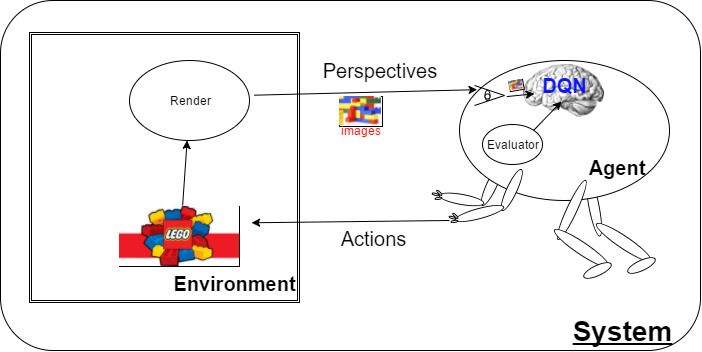
\includegraphics[width=\textwidth]{agent_env.png}
                \caption{Overall System.}
                \label{fig:system1}
            \end{figure}
            
            The environment consists of a simulated LEGO environment and a renderer. The simulated LEGO environment offers the agent actions. According to the action commands sent from the agent, LEGO models can be rigged up in the simulated LEGO environment. The simulated LEGO environment can also import a model from a \textit{.lxfml} or \textit{.lxf} file, or export the current model to a \textit{.lxfml} or \textit{.lxf} file. The renderer can then input a \textit{.lxfml} or \textit{.lxf} file, and then render the model into an image which can be perceived by the agent. 
            
            The agent consists of a reward function, a deep Q-network and a replay (experience) pool. The reward function evaluates the difference between the model which the agent has already rigged up and the target model. The deep Q-network is the core of the whole algorithm, which tells the agent Q-values of each action at each state. Replays (experiences) in the pool can be randomly picked to train the network. 
            
            The inter-communication between modules can be illustrated by Figure~\ref{fig:inter-communication}. 
            
            \begin{figure}[h]
                \centering
                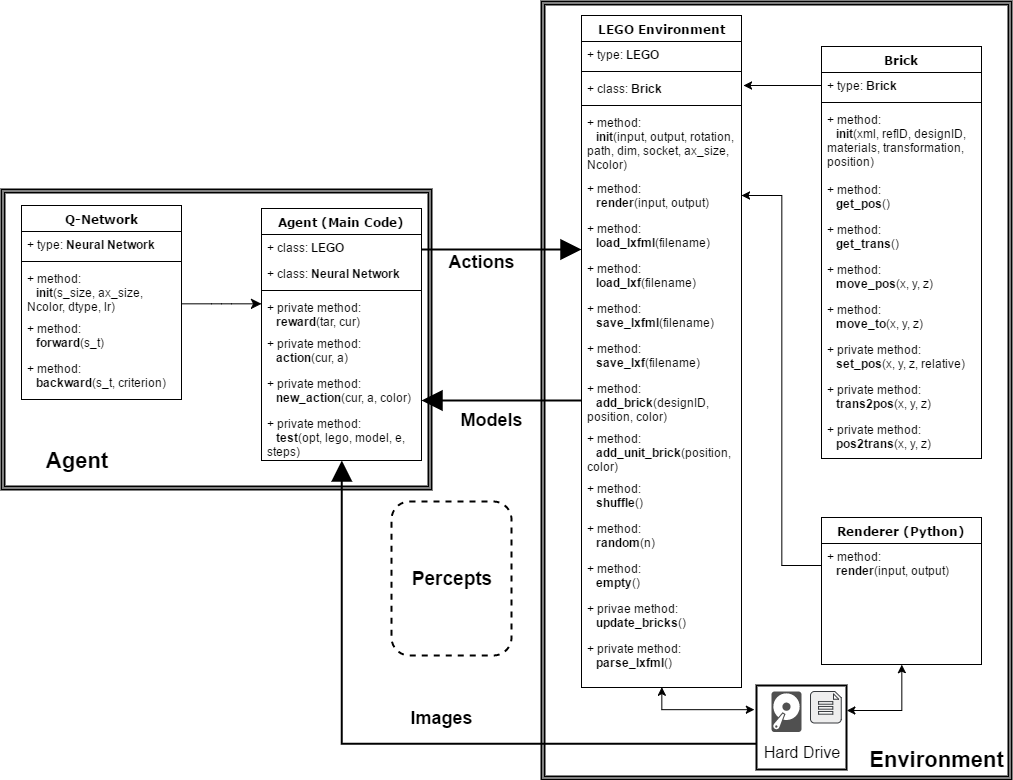
\includegraphics[height=0.99\textwidth, angle=-90]{inter-communication.png}
                \caption{Inter-Communication between modules.} 
                \label{fig:inter-communication}
                
            \end{figure}
        
	        The communication between the agent and the environment is based on both memory and hard drive. Model files (\textit{.lxfml} and \textit{.lxf} files) and rendered images are stored on the hard drive.
	        
	        
            
            
            
            
            

            

            
            
            
            
            
            % \let\labelitemi\labelitemii

            % \begin{itemize}
            %   \item adding a brick at a specific coordinates
            %   \item moving a brick to a specific coordinates
            %   \item 
            % \end{itemize}
            % adding a brick at a specific coordinates, moving a brick to a specific coordinates
            

        
        
        \subsection{Agent}
	        \subsubsection{Early Stage}
		        In the early stage of the project, the LEGO environment was only in 2D. The agent could only move bricks in a 2D plane. All the interrelated images in this stage have 3 channels (RGB).
		        
		        The main code of the agent is shown by Algorithm~\ref{alg:lego1} and the corresponding testing procedure is shown by Algorithm~\ref{alg:test1}. 
		        
		        \begin{algorithm}[]
		        	\caption{LEGO with deep Q-learning (at the early stage)} \label{alg:lego1}
		        	\begin{algorithmic}[1]
		        		\State Require hyper-parameters
		        		\State Initialise replay memory $D$ to capacity $N$
		        		\State Initialise action-value function $Q$ with random weights $\theta$
		        		\State Initialise target action-value function $\hat{Q}$ with weights $\theta^- = \theta$
		        		\State Input a target model $M_{target}$ to the agent and the environment
		        		\State Initialise a neural network $Net$ with random parameters
		        		\State Initialise Q-values for each state-action pair
		        		
		        		
		        		\For {$episode = 1, N\_episode$}
		        		\State Generate an initial model $M_1$ in the environment
		        		\State The agent gets the initial model $M_1$ from the environment
		        		\State Acquire an image $x_1$ of $M_1$ from the environment
		        		\State Initialise sequence $s_1 = {M_1}$
		        		\For{$t=1,N$}
			        		\State Pass $x_t$ to $Net$ to get Q-values $Q$
			        		\State With probability $\epsilon$ select a random action $a_t$
			        		\State otherwise select $a_t = \argmax_a Q(s_t, a;\theta)$
			        		\State Translate the selected action $a_t$ to a command $(brick, axis, direction)$
			        		\State Pass the command $(brick, axis, direction)$ to the environment
			        		\State Acquire the next model $M_{t+1}$ and a corresponding image $x_{t+1}$
			        		\State Pass $M_{target}$ and $M_{t+1}$ to the reward function
			        		\State Get a reward $r_t$ and a terminating flag $terminate_{t+1}$
			        		\State Store transition ($x_t,a_t,r_t,x_{t+1}$) in $D$
			        		\State Sample random mini-batch of transitions ($x_t,a_t,r_t,x_{t+1}$) from $D$
			        		\State Set $
				        		y_j= 
				        		\begin{cases}
				        		r_j    & \parbox[t]{.15\textwidth}{\text{episode terminates at step } j+1}\\
				        		r_j+\gamma\max_{a'}\hat{Q}(x_{j+1},a';\theta^-) & \text{otherwise}
				        		\end{cases}
				        		$
			        		\State Perform a gradient descent step on $(y_j-Q(x_j,a_j;\theta))^2$ with respect
			        		\StatexIndent[2] to the network parameters $\theta$
			        		\State Every $C$ steps reset $\hat{Q} \gets Q$
			        		\State Store statistics
			        		\If {$terminate_{t+1}$}  
			        			\State Break the loop 
			        		\EndIf
		        		
		        		\EndFor
		        		
		        		\State Every $N\_test$ episodes, \textbf{Test(\text{$M_{target}, Net$})}

		        		\State Store statistics 

		        		\EndFor
		        	\end{algorithmic}
		        \end{algorithm}
		        
		        \begin{algorithm}[]
		        	\caption{Testing procedure (at the early stage)} \label{alg:test1}
		        	\begin{algorithmic}[1]
		        		\Procedure{\textbf{Test}}{$M_{target}, Net$}
		        		\State Pass the target model $M_{target}$ to the environment
		        		\State Generate an initial model $M_1$ in the environment
		        		\State The agent gets the initial model $M_1$ from the environment
		        		\State Acquire an image $x_1$ of $M_1$ from the environment
		        		\For{$t=1,N$}
		        		\State Pass $x_t$ to $Net$ to get Q-values $Q$
		        		\State Select $a_t = \argmax_a Q(s_t, a;\theta)$
		        		\State Translate the selected action $a_t$ to a command $(brick, axis, direction)$
		        		\State Passes the command $(brick, axis, direction)$ to the environment
		        		\State Acquire the next model $M_{t+1}$ and a corresponding image $x_{t+1}$
		        		\State Pass $M_{target}$ and $M_{t+1}$ to the reward function
		        		\State Get a reward $r_t$ and a terminating flag $terminate_{t+1}$
		        		\State Store the statistics
		        		\If {$terminate_{t+1}$}  
		        		\State Break the loop 
		        		\EndIf
		        		
		        		\EndFor
		        		\EndProcedure
		        	\end{algorithmic}
		        \end{algorithm}
		        
		        Initially, a target model is required from the user. Then $N\_episode$ episodes will be processed. 
		        
		        In each episode, the environment first generates a initial model $M_1$ which consists of every brick in the target model in random positions, and passes it to the agent. The agent then calls the \textbf{render} method and reads an rendered image $x_1$ of $M_1$ from the hard drive. 
		        
		        \vspace{5mm}
		        
		        Then the agent will repeat the following processes in $N$ steps or the agent finishes to build the model. 
		        
		        At each time step $t$, the agent first passes the rendered image $x_t$ to the network, and gets Q-values $Q$. It then select the action with the highest Q-value in the action space, and translates it to a command $(brick, axis, direction)$. Each command stands for `moving a $brick$ along either x-axis or y-axis in a $direction$ by a unit distance'. The action space $A$ has a cardinality of $|Bricks| \times 2 \times 2$. This command will be inputted into the environment by the \textbf{move\_pos} method. The environment changes the model to $M_{t+1}$ correspondingly, and the agent can get the model $M_{t+1}$ and the rendered image $x_{t+1}$. The agent passes the target model $M_{target}$ and the $M_{t+1}$ to the reward function and get a reward $r_t$ and a terminating flag $terminate_{t+1}$. 
		        
		        The reward function here calculates the difference in distance for each identical brick in the target model $M_{target}$ and the next model $M_{t+1}$, and returns the negative sum of distances as the reward value $r_t$ and a terminating flag $terminate_{t+1}$. The reward value is negative because we want the reward value becomes negatively large if the difference in distances is large.
		        
		        \begin{equation*}
			        reward(M_{target}, M_{t+1}) = - \sum_{brick \in M_{target}} ||coor_{M_{target}}(brick) - coor'_{M_{t+1}}(brick)||
		        \end{equation*} 
		        
		        \begin{equation*}
			        terminate_{t+1} = (M_{target} == M_{t+1})
		        \end{equation*}
		        
		        Then the agent stores the experience ($x_t,a_t,r_t,x_{t+1}$) in $D$. If there are enough experiences in $D$, the agent uniformly draws some experiences and performs a gradient descent step to the network. 
		        
		        Then the loop will continue if the agent was unable to build the target model. If the agent managed to do so, the next episode will start. 
		        
		        \vspace{5mm}
		        
		        For every $N_{test}$ episodes, the agent may test itself using the currently trained network. In order to increase time efficiency, I set $N_{test}$ to a high value.
		        
		    \subsubsection{3D}
		    	After the early stage, I expand the render so a 3D environment is supported. The main code doesn't change too much except that the action space $A$ is expanded and the cardinality of $A$ becomes $|Bricks| \times 3 \times 2$, since the agent may move a brick along the z-axis. The related images are expanded to 4 channels (RGB channels and a depth channel), so the agent can detect the relative depth of each pixel in an image.  
		    	
        	\subsubsection{Reward Function}
        		The initial reward function was limited as it takes two models as arguments. The whole system was therefore restricted so that the agent could only imitate a LEGO model. In order to broke through, I tried some different reward functions which were based on image comparison. The final reward function I used was TV-L1\cite{tvl1}. 
        		
        		TV-L1 is an optical flow algorithm which detects movements of objects in two images. I found it working well in finding the movements of bricks. The algorithm returns a pair of matrices $(magnitude, angle)$, where $magnitude$ is a matrix which, for each pixel, gives a magnitude of the movement between 0 and 1, and $angle$ is a matrix which, for each pixel, gives a vector representing the direction of movement. The reward function sums up the matrix $magnitude$ and return the sum as the reward value. 
        		
        		Now the agent has the ability of comparing a real-world image and a rendered image of a LEGO model. 
        		
        		Even though this algorithm works well, we still need to explore and find some other algorithms as the reward function which works better than this algorithm, as finding a good reward function is a major task in reinforcement learning. Due to the time limitation of this project, I couldn't try many algorithms. However, I have some ideas in mind and I will show them in the `Future Works' section. 
        		
        	\subsubsection{Final Stage}
        		The time efficiency is a huge problem in machine learning. The whole system worked, but it was extremely time consuming. It took thousands of episodes to train an agent to play with 3 or 4 bricks. And the total time cost was several days. Then I pondered the whole system. I realised that moving one unit distance in each time step was very inefficient. Moreover, the action space was also too large. The action space is in $O(bricks)$. This also leads to an extraordinary large amount of parameters in the network if the number of bricks increases. 
        		
        		In order to break through the problem, I tried to analyse the way when people playing with LEGO. The whole system so far is in a similar way where people buy a box of LEGO bricks and build a model using bricks in the box. The target model is the one printed on the box. The box contains every brick required to build the target model and normally there is no extra brick. However, this is not the way when LEGO experts build LEGO models. The experts normally have a large pool of bricks with different shape and colours. What they need to do is to find a brick with the best shape and the best colour and put it to the best position. 
        		
        		As a result, I tried to fix the system so that there are unlimited bricks offered to the agent to build models (due to the restriction of the environment, I could only simulate unit bricks, so the unlimited bricks are unit bricks of all colour available in the LEGO Digital Designer). In this case, however, the action space is no longer depending on the number of bricks, but on the number of colours and the number of positions to place bricks. As there are limited number of colours and positions, the action space doesn't change when the number of bricks increases. 
        		
        		The algorithm after upgrade is shown by Algorithm~\ref{alg:lego2}, and the corresponding testing procedure is shown by Algorithm~\ref{alg:test2}.
        		
        		\begin{algorithm}[]
        			\caption{LEGO with deep Q-learning (at the final stage)} \label{alg:lego2}
        			\begin{algorithmic}[1]
        				\State Require hyper-parameters
        				\State Initialise replay memory $D$ to capacity $N$
        				\State Initialise action-value function $Q$ with random weights $\theta$
        				\State Initialise target action-value function $\hat{Q}$ with weights $\theta^- = \theta$
        				\State Input a target model $M_{target}$ to the agent and the environment
        				\State Render $M_{target}$ into $x_{target}$
        				\State Initialise a neural network $Net$ with random parameters
        				\State Initialise Q-values for each state-action pair
        				
        				
        				\For {$episode = 1, N\_episode$}
	        				\State Generate an initial model $M_1$ in the environment
	        				\State The agent gets the initial model $M_1$ from the environment
	        				\State Acquire an image $x_1$ of $M_1$ from the environment
	        				\State Initialise sequence $s_1 = {M_1}$
	        				\For{$t=1,N$}
%		        				\State Pass $x_t$ to $Net$ to get Q-values $Q$
%		        				\State With probability $\epsilon$ select a random action $a_t$
		        				\If {rand() $< \epsilon $}
		        					\State select a random action $a_t$
		        				\Else
		        					\For {$colour \in C$}
		        						\State Encode $colour$ into one-hot encoding $colour'$ 
		        						\State Combine $colour'$ and $x_t$ to $x'_t$
		        						\State Pass $x'_t$ to $Net$ to get Q-values $Q$
		        					\EndFor
		        					\State Select $a_t = \argmax_{coor,colour} Q(s_t, coor, colour;\theta)$
		        				\EndIf
		        				\State Pass the command $(coor, colour)$ to the environment
		        				\State Acquire the next model $M_{t+1}$ and a corresponding image $x_{t+1}$
		        				\State Pass $x_{target}$ and $x_{t+1}$ to the reward function
		        				\State Get a reward $r_t$ and a terminating flag $terminate_{t+1}$
		        				\State Store transition ($x_t,a_t,r_t,x_{t+1}$) in $D$
		        				\State Sample random mini-batch of transitions ($x_t,a_t,r_t,x_{t+1}$) from $D$
		        				\If {episode terminates at step $j+1$}
		        					\State $y_j \gets r_j$
		        				\Else
		        					\State $y_j \gets r_j+\gamma\max_{coor', colour'}\hat{Q}(x_{j+1},coor', colour';\theta^-)$
		        				\EndIf
		        				\State Perform a gradient descent step on $(y_j-Q(x_j,a_j;\theta))^2$ with respect
		        				\StatexIndent[2] to the network parameters $\theta$
		        				\State Every $C$ steps reset $\hat{Q} \gets Q$
		        				\State Store statistics
		        				\If {$terminate_{t+1}$}  
		        					\State Break the loop 
		        				\EndIf
	        				
	        				\EndFor
	        				
	        				\State Every $N\_test$ episodes, \textbf{Test(\text{$M_{target}, Net$})}
	        				
	        				\State Store statistics 
        				
        				\EndFor
        			\end{algorithmic}
        		\end{algorithm}
        		
        		\begin{algorithm}[]
        			\caption{Testing procedure (at the final stage)} \label{alg:test2}
        			\begin{algorithmic}[1]
        				\Procedure{\textbf{Test}}{$M_{target}, Net$}
        				\State Pass the target model $M_{target}$ to the environment
        				\State Render $M_{target}$ into $x_{target}$
        				\State Generate an initial model $M_1$ in the environment
        				\State The agent gets the initial model $M_1$ from the environment
        				\State Acquire an image $x_1$ of $M_1$ from the environment
        				\For{$t=1,N$}
	        				\For {$colour \in C$}
		        				\State Encode $colour$ into one-hot encoding $colour'$ 
		        				\State Combine $colour'$ and $x_t$ to $x'_t$
		        				\State Pass $x'_t$ to $Net$ to get Q-values $Q$
	        				\EndFor
	        				\State Select $a_t = \argmax_{coor,colour} Q(s_t, coor, colour;\theta)$
	        				\State Passes the command $(coor, colour)$ to the environment
	        				\State Acquire the next model $M_{t+1}$ and a corresponding image $x_{t+1}$
	        				\State Pass $x_{target}$ and $x_{t+1}$ to the reward function
	        				\State Get a reward $r_t$ and a terminating flag $terminate_{t+1}$
	        				\State Store the statistics
	        				\If {$terminate_{t+1}$}  
	        					\State Break the loop 
	        				\EndIf
	        				
        				\EndFor
        				\EndProcedure
        			\end{algorithmic}
        		\end{algorithm}
        	
        	
        		In this algorithm, instead of directly passing an image to the network, it iterates over colour space, combine the colour index and the image together and then pass the processed image to the network. The network returns Q-values for each coordinates with respect to a colour. Then the agent selects a colour and a coordinate with the maximum Q-value as the action. The action in this algorithm is a pair of coordinates and colour. Each action pair $(coor, pair)$ stands for adding a unit brick with colour $colour$ to the model at $coor$, so the size of the action space is $|C|\times {ax\_size^3}$, where $ax\_size$ is the number of discrete positions on which bricks can be put along one axis. 
        		
        		This algorithm was later experimented by several tests, and the tests turned out that the algorithm worked as I thought, since the agent could now build models with dozens of bricks. 
        		
        		\newpage
        		
        		
        
        \subsection{Deep Q-Network}
            
            In the first stage of the project, the Q-network is much simpler than it in the later stage. The network takes an image with 3 channels as an input, and outputs Q-values for each action. The network consists of an input layer, a hidden layer, several convolutional hidden layers and some other necessary hidden layers. 
            
            In the later stage of the project, in addition to the image, the network also takes an one-hot encoded value, representing the index of the colour of a brick to be added into the model. For example, if the agent tries to add a red brick where the index of red is 2, the input is an image of current state and a one-hot encoded value $010...0$. The output of the network also changes. This time, there are three output layers. Each layer represents the coordinate on an axis, so the three layers together give the coordinates which a brick of the colour should be put on. 
        
        
        \subsection{LEGO Environment}
        
        	\subsubsection{Brick}
        
        
        \subsection{Renderer}
        
            Since I am using Blender to render and Blender only supports Python, the renderer is written in Python and the other modules can call the renderer through command line and transfer files using hard drive or network socket. 
            
            In order to save memory, and for convenience, I extracted every brick's 3D model from the LEGO digital designer and saved them as \textit{.obj} files on hard drive. I also stored some colour information and texture information for each kind of simple bricks into a table. When the renderer needs to render a specific brick with a specific colour or texture, it can import the corresponding \textit{.obj} file from the disk and fetch the texture from the table. 
            
            
        
        
    
    \section{Testing}
    
    \section{Results}
    
    \section{Conclusions}
    
        \subsection{Future Works}
        
        \subsection{Personal Report}
    
    \section{Acknowledgements}
    
    \section{Appendices}
    
    \bibliographystyle{alpha}
    \bibliography{LEGO}
    \nocite{*}
    



\end{document}
